\headerblock{
  \headerquote{Well-chosen, non-frivolous epigraphs can enhance a thesis.}{Dave Clarke~\cite{AcademiaSE}}

  % \headerbreak{}
  %
  % \headerhide{
  %   \headerimage{img/latte.jpg}
  % }
}

\section{Epigraph Outtakes}

\headerblock{
\headerquote{Elegance is not a dispensable luxury but a quality that decides between success and failure.}{Edsger Dijkstra}

\headerquote{The restriction of finiteness appears to give a better approximation to the idea of a physical machine. Of course, such machines cannot do as much as Turing machines, but the advantage of being able to compute an arbitrary general recursive function is questionable, since very few of these functions come up in practical applications.}{Rabin and Scott}

\headerquote{Almost every problem that you come across is befuddled with all kinds of extraneous data of one sort or another; and if you can bring this problem down into the main issues, you can see more clearly what you’re trying to do.}{Claude Shannon}

\headerquote{Definitions belong to the definers, not the defined.}{Toni Morrison}

\headerquote{caleb i swear to god if you don’t finish this dissertation i will personally order one of the cats to attack you}{Russell}
}

\section{Image Outtakes}

\begin{center}
  \headerimage{img/xkcd-standards.png}
\end{center}

\section{Special Thanks}

\begin{center}
  \setlength{\tabcolsep}{10pt}
  \renewcommand{\arraystretch}{3.3}
  \begin{tabular}{cc}
    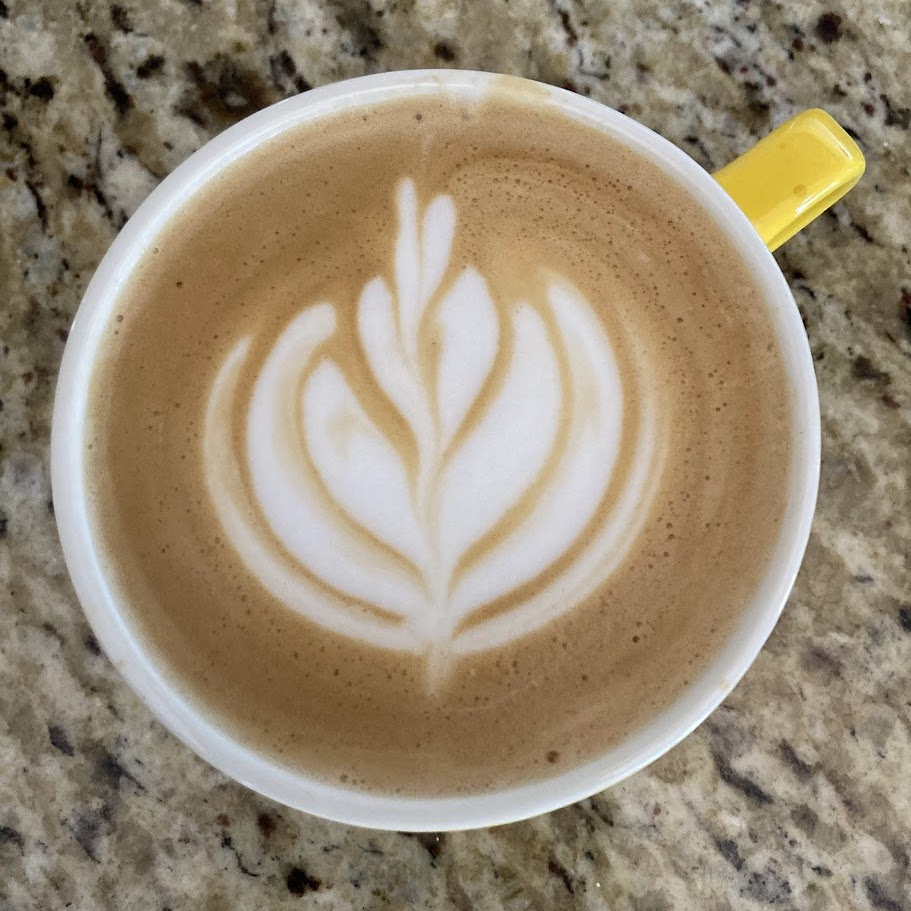
\includegraphics[width=6cm]{img/latte-06-26.jpg} &
    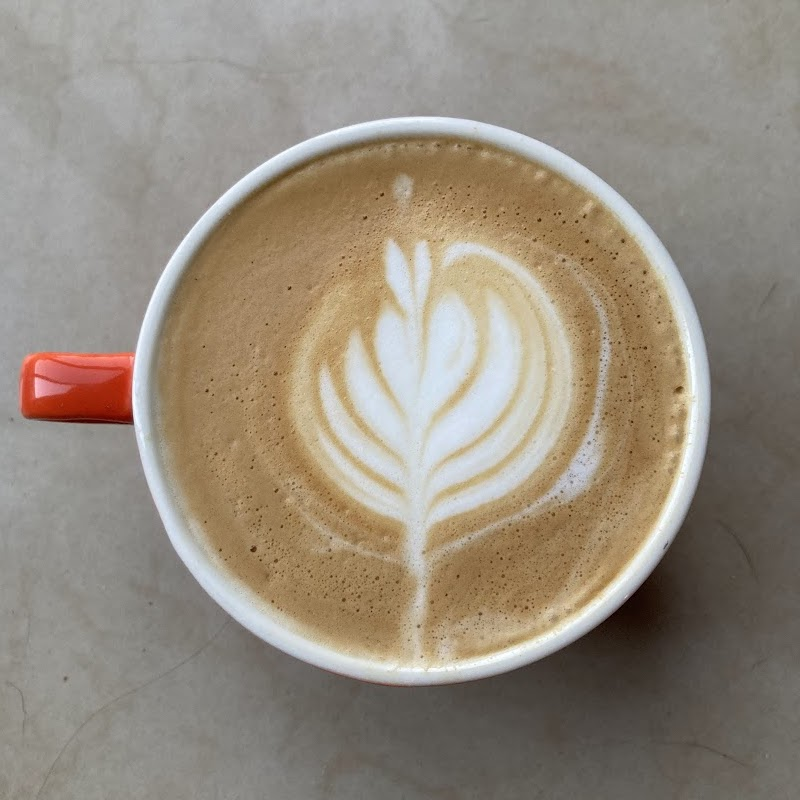
\includegraphics[width=6cm]{img/latte-06-29.jpg} \\
    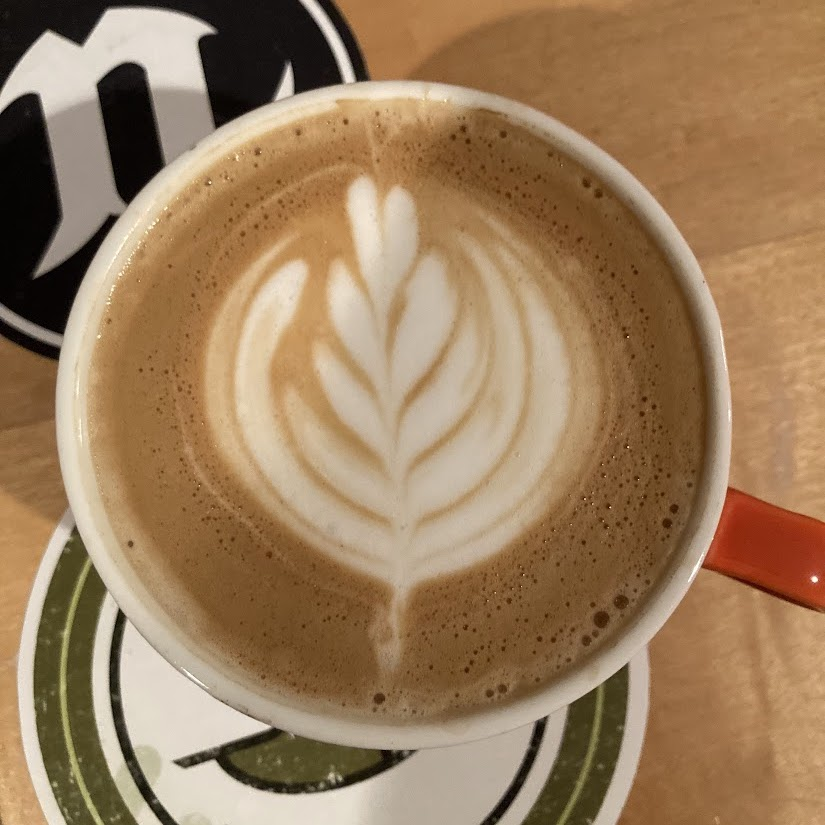
\includegraphics[width=6cm]{img/latte-07-02.jpg} &
    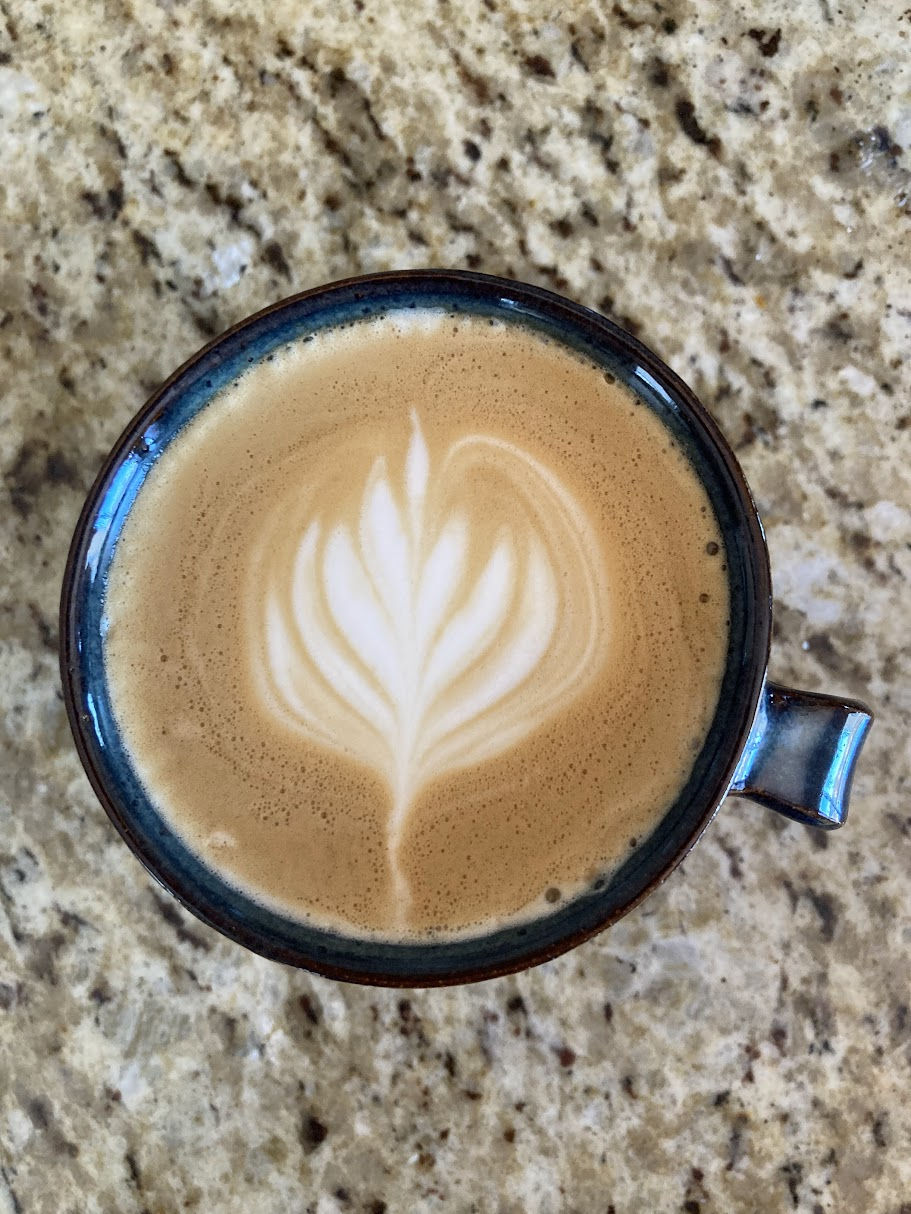
\includegraphics[width=6cm]{img/latte-07-04.jpg} \\
  \end{tabular}
\end{center}
